\documentclass{article}


\usepackage{arxiv}

\usepackage[utf8]{inputenc} % allow utf-8 input
\usepackage[T1]{fontenc}    % use 8-bit T1 fonts
\usepackage{hyperref}       % hyperlinks
\usepackage{url}            % simple URL typesetting
\usepackage{booktabs}       % professional-quality tables
\usepackage{amsfonts}       % blackboard math symbols
\usepackage{nicefrac}       % compact symbols for 1/2, etc.
\usepackage{microtype}      % microtypography
\usepackage{lipsum}		% Can be removed after putting your text content
\usepackage{textgreek}
\usepackage{amsmath}
\usepackage{algorithm}
\usepackage{algpseudocode}
\usepackage{algpascal}
\usepackage{graphicx}
\usepackage[
backend=biber,
style=numeric,
sorting=ynt,
citestyle=authoryear
]{biblatex}
\addbibresource{paper.bib}

%\graphicspath{ {./images/} }

\title{Lunar Lander with Deep Reinforcement Learning}

\date{June 30th, 2019}

\author{
Carlos Souza\thanks{Latest Git hash: INCLUDE LATEST GITHASH}\\
%Department of Computer Science\\
Georgia Institute of Technology\\
%São Paulo, SP, Brazil \\
\texttt{souza@gatech.edu} \\
}

\DeclareMathOperator*{\argmax}{arg\,max}
\DeclareMathOperator*{\argmin}{arg\,min}


\begin{document}
    \maketitle

    % keywords can be removed
    %\keywords{Reinforcement learning \and Deep Reinforcement Learning \and Deep Q-Networks}
    %\githash{DO NOT FORGET TO INCLUDE LATEST GIT HASH}


    \section{Introduction}
    \label{sec:introduction}
    Reinforcement learning (RL) theory provides mathematical background and classic algorithms to enable agents to learn optimally control an environment.
    However, to successfully apply those algorithms in problems with real-world complexity, several challenges must be tackled, must notably i) how to derive efficient representations of the environment from high-dimensional sensory inputs, and ii) how to use these to generalize past experience to new situation (\cite{dqn}).

    Recent advances in deep neural networks (DNNs) originated a new type of agent, known as Deep Q-Network agent, capable of overcoming these challenges, which enabled RL algorithms to perform effectively.
    All the many recent successes in applying RL to complex sequential decision-making problems were kick-started by the Deep Q-Network algorithm (DQN; \cite{dqn}).
    Since then, many extensions have been proposed to improve its stability and/or speed.
Double DQN (DDQN; \cite{ddqn}) addresses the problem of overestimation of action values, by decomposing the max operation in the target into action selection and action evaluation.
    The Dueling Network architecture (Dueling DDQN; \cite{dueling}) better generalize learning accross actions by proposing an architecture that explicitly separates the representation of state values and (state-dependent) action advantages.
    Prioritized Experience Replay (PER; \cite{per}) improves data efficiency, by replaying more often transitions from which there is more to learn.

    Each of these algorithms enables substantial performance improvements in isolation and combined, since they build on a shared framework.
    In this paper we propose to study an agent that combines all the aforementioned improvements, exploring its performance in Lunar Lander environment from OpenAI gym (\cite{openai}).

    \subsection{Background}
    \label{subsec:background}
    One of the early breakthroughs in RL was the development of an off-policy Temporal Difference control algorithm known as \emph{Q-learning} (\cite{qlearning}), defined by:
    \begin{equation}
        Q(s_{t}, a_{t}) \leftarrow Q(s_{t}, a_{t}) + \alpha \left[ r_{t+1} + \gamma \max_{a} Q(s_{t+1}, a) - Q(s_{t}, a_{t}) \right],
    \end{equation}
    where $\alpha$ is a constant step-size parameter, or learning rate.
    The learned action-value function $Q$ directly approximates the \emph{optimal} action-value function $Q^{*}$, independent of the policy being followed.

    However, large state and/or action spaces make it intractable to learn $Q$ value estimates for each state-action pairs independently.
    To solve this challenge, DQN (\cite{dqn}) successfully used deep neural networks to approximate the state-action value function as $Q(s, a; \theta)$, where $\theta$ are the parameters of the network.
    For an $n$-dimensional state space and an action space containing $m$ actions, the neural network is a function from $\mathbb{R}^{n}$ to $\mathbb{R}^{m}$.

    Two important components of the DQN algorithm proposed by \cite{dqn} are i) the use of a target network, and ii) the use of experience replay.
    At each time step, the agent selects an action $\epsilon$-greedily with respect to the action values, and adds a transition $\langle s_{t}, a_{t}, r_{t}, s_{t+1} \rangle$ to the experience replay memory, that holds millions of experience tuples.
    The parameters of the neural network are then optimized by using stochastic gradient descent to minimize the loss function at iteration $i$:
    \begin{align}
        L_{i}(\theta_{i}) &= \mathbb{E}_{s, a, r, s'} \left[ \left( y_{i} - Q(s, a; \theta_{i}) \right)^2 \right] \\
        y_{i} &= r + \gamma \max_{a'}Q(s', a'; \theta^{-})
    \end{align}
    where $\theta^{-}$ are the parameters of a fixed and separate \emph{target network}.
    The parameters of the target network $Q(s', a'; \theta^{-})$ are frozen for a fixed number of iterations while updating the \emph{online network} $Q(s, a; \theta_{i})$ by gradient descent.
    The optimization is performed on mini-batches sampled uniformly at random from the experience replay memory.
    These two additions greatly improves the stability of the algorithm, leading to super-human performance on several Atari games.

    \subsection{DQN Extensions}
    \label{subsec:extensions}

    \paragraph{Double Q-learning.}
    The max operator in standard Q-learning and DQN uses the same values both to select and to evaluate an action.
    This makes it more likely to select overestimated values, resulting in overoptimistic value estimates.
    To prevent this, we can decouple the selection from the evaluation.
    This is the idea behind Double Q-learning.
    It is possible to effectively combine this with DQN using the loss
    \begin{align}
        L_{i}(\theta_{i}) &= \mathbb{E}_{s, a, r, s'} \left[ \left( y_{i} - Q(s, a; \theta_{i}) \right)^2 \right] \\
        y_{i} &= r + \gamma Q(s', \argmax_{a'} Q(s', a'; \theta_{i}); \theta^{-}),
    \end{align}
    which was shown to improve performance by reducing value overestimates present in vanilla DQN.

    \paragraph{Dueling networks.}
    The dueling network is a DNN architecture designed for value based RL.
    The key insight behind it is that, for many states, it is unnecessary to estimate the value of each action choice.
    After the first DQN original layers, two streams of fully-connected layers are constructed such that they have the capability of providing separate estimates of the value and advantage functions, being the \emph{advantage function} defined as $A^{\pi}(s, a) = Q^{\pi}(s, a) - V^{\pi}(s)$.
    Finally, the two streams are combined to produce a single output $Q$ function
    \begin{equation}
        Q(s, a; \theta, \alpha, \beta) = V(s; \theta, \beta) + \left( A(s, a; \theta, \alpha) - \frac{1}{|\mathcal{A}|} \sum_{a'} A(s, a'; \theta, \alpha) \right),
    \end{equation}
    where $\theta$ denotes the parameters of the previous layers, while $\alpha$ and $\beta$ are the parameters of the two streams of fully-connected layers.
    As the dueling architecture shares the same input-output interface with standard Q networks, we can recycle all learning algorithms with Q networks to train the dueling architecture.

    \paragraph{Prioritized experience replay.}
    DQN samples uniformly from the replay memory.
    Their key idea behind prioritized experience replay is to increase the replay probability of experience tuples from which there is much to learn.
    \cite{per} proposes the last encountered absolute \emph{TD error} as a proxy for learning potential, which is the central component of the algorithm.

    Several implementation challenges arise from the greedy TD-error prioritization and the bias it introduces by changing the distribution of experience samples.
    To overcome those, the algorithm implements \emph{stochastic prioritization} and \emph{weighted importance-sampling}.

    Prioritized experience replay is shown to deliver both faster learning and better final policy quality across most games of the Atari benchmark suite, as compared to uniform experience replay.

    \section{Methods}
    \label{sec:methods}
    To investigate how the integrated agent that combines all described improvements perform, using Lunar Lander environment as test-bed, we propose 5 different experiments detailed below.

    \paragraph{Experiment 1: Impact of different learning protocols and DQN extensions.}
    We started our study by analyzing the impact of two learning protocols in 8 different agents.
    In the first learning protocol, agents kept learning for 1000 episodes.
    In the second, we stopped the learning as soon as 100-episodes rolling average of the score hit 200, acting greedily from that point on until reaching 1000 episodes, for comparison.
    The 8 different agents combine all DQN extensions, representing all possible combinations.
    The simplest agent implements vanilla DQN, while the most sophisticated, the integrated agent, combines all extensions described earlier.
    We also compared these with agents containing only one and/or two extensions, to understand the impact of each extension on their performance.

    While varying the extensions, we kept all other hyper-parameters frozen.
    We used RMSProp as the optimization algorithm, with $\alpha$ (learning rate) of $0.0001$.
    $\gamma$ (discount factor) was set at $0.99$.
    Replay memory capacity was set to $10,000$ experience tuples, and training was performed using $32$ as mini-batch size.
    The network architecture consists of 2 fully-connected hidden layers with 512 neurons each, both with rectified linear unit (ReLU) activation functions (for dueling network: we added a fully-connected layer as described previously).
    For prioritized replay, we annealed the bias by progressively increasing $\beta$ (exponent in importance-sampling weights) from $0.4$ to $1$.
    As exploration strategy, we decayed $\epsilon$ following $\epsilon(t) = e^{-t/70}$, where $t$ is the current episode, until hitting $0.05$, staying constant at $0.05$ from that point on.

    To reduce the variability given the stochasticity, this experiment was performed 20 times for each variant.

    \paragraph{Experiment 2: Effect of different gradient descent optimization algorithms and learning rates.}
    Next, we assessed the effect of different optimization algorithms and their optimal learning rates on the integrated agent, which combines all DQN extensions.
    We simulated RMSProp, Adaptive Moment Estimation (Adam), and Stochastic Gradient Descent (SGD).
    For those 3 different algorithms, we tested $30$ different $\alpha$ (learning rates), evenly spaced on a log scale from $10^{-6}$ to $10^{-1}$.
    All other hyper-parameters were kept frozen as described in experiment 1.

    \paragraph{Experiment 3: Discount factor sensitivity.}
    In this experiment, we investigated the effect of $\gamma$ in the integrated agent's performance.
    We tested all $\gamma \in [0.8, 0.85, 0.9, 0.92, 0.94, 0.96, 0.98, 0.99, 1.0]$.
    As usual, all other hyper-parameters were kept frozen.
    To reduce the variability given the stochasticity, this experiment was performed 5 times for each variant.

    \paragraph{Experiment 4: Evaluation of different exploration strategies.}
    Following, we evaluated the impact of $10$ different $\epsilon$ decay curves.
    We assessed two types of curves: exponential decay functions, $\epsilon(t) = e^{-k t}$; and inverted logistic functions, $\epsilon(t) = 1 / (1 + e^{-k_{1} (t - k_{2})})$.
    Again, all other hyper-parameters were kept frozen.
    To reduce the variability given the stochasticity, this experiment was performed 10 times for each variant.

    \section{Results}
    \label{sec:results}

    \begin{figure}[t]
        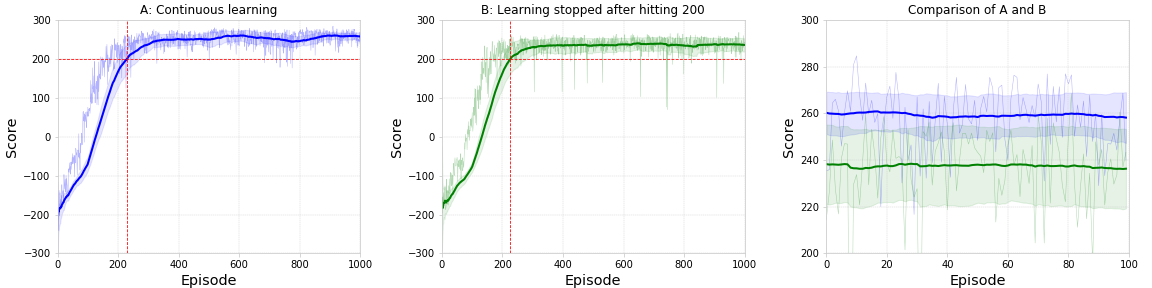
\includegraphics[width=\textwidth]{./images/fig1.png}
        \centering
        \caption{Different learning protocols.
        In the left, integrated agent (combining all DQN extensions) learns continuously for 1000 episodes.
        In the center, integrated agent learns just until it achieves 200 score over 100-episodes rolling average, acting greedily from that point on until 1000 episodes.
        In the right, we test both learning protocols, comparing both trained agents (no learning).
        All results presented are averages of 20 runs to reduce the variance: the shaded area is the standard deviation.}
        \label{fig:fig1}
    \end{figure}

    Figure \ref{fig:fig1} presents first part of experiment 1, in which we confirmed our expectations.
    In both learning protocols, the integrated agent, combining all DQN extensions, solved Lunar Lander environment by reaching 200 score over past 100-episodes rolling average around the same time, in 230 and 226 episodes respectively.
    Also, as expected, the learning protocol that kept the agent learning for the whole 1000 episodes achieved a higher score in the 100-episodes test, 259 in average, in comparison to the learning protocol that stopped the learning after solving the environment (only 237 in average).

    \begin{figure}[h]
        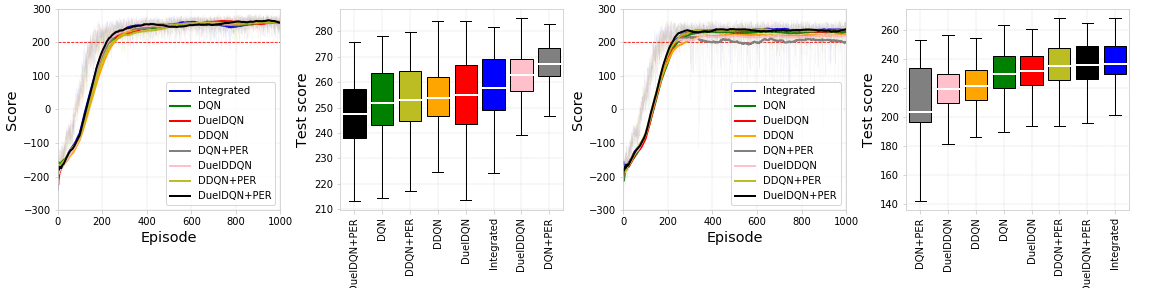
\includegraphics[width=\textwidth]{./images/fig2.png}
        \centering
        \caption{Different agents.
        The 2 charts in the left show the first learning protocol, where agents keep learning for 1000 episodes, while the 2 charts in the right show the second learning protocol, where agents stop learning right after reaching 200 score on 100-episodes rolling average.
        To better visualize the test score results, comparing the performance of all different agents over 100 episodes with no learning, in second and fourth chart we used boxplots, for the first and second learning protocols respectively.}
        \label{fig:fig2}
    \end{figure}

    Figure \ref{fig:fig2} presents second part of experiment 1.
    First 2 charts show first learning protocol (all agents keep learning for 1000 episodes), while last 2 charts show second learning protocol (agents stop learning as soon as they hit 200 score).
    Regardless of the learning protocol, all agents solve Lunar Lander environment in 200 to 250 episodes.

    In the first learning protocol, the agent with the second worst performance was the vanilla DQN, with 251 score over 100-episodes test, contradicting our expectation: we expected this agent to show the poorest performance.
    The agent with the worst performance implemented DQN with Dueling Networks and Prioritized Experience Replay (DuelDQN+PER).
    Also contradicting our expectation, two agents showed better performance than the integrated agent (257 score): the agent with Dueling Networks + Double DQN (DuelDDQN, with 263 score), and the DQN agent with Prioritized Experience Replay (DQN+PER, with 267 score).

    In the second learning protocol, the best agent was the integrated agent (237 score), which combines all DQN extensions, confirming our expectation.
    However, contradicting our expectation, in this case the worst performance was not the vanilla DQN, but surprisingly the DQN agent with Prioritized Experience Replay (PER, with 204 score), which had performed best in the first learning protocol.

    These results suggest that the integrated agent is the best choice in limited/short training time, as it scored the highest amongst all options when learning happened only until 100-episodes rolling average hit 200 score.
    They also suggest that the Prioritized Experience Replay extension benefit is only perceived when learning happens for longer.
    Another interesting observation is regarding the agent with Double DQN and Prioritized Experience Replay (DDQN+PER).
    It performed second worse in first learning protocol, but second best in second learning protocol, which suggests those extensions, combined, are great tools to improve the performance in limited training time, but are not as interesting when we have time to train for longer periods.

    \begin{figure}[t]
        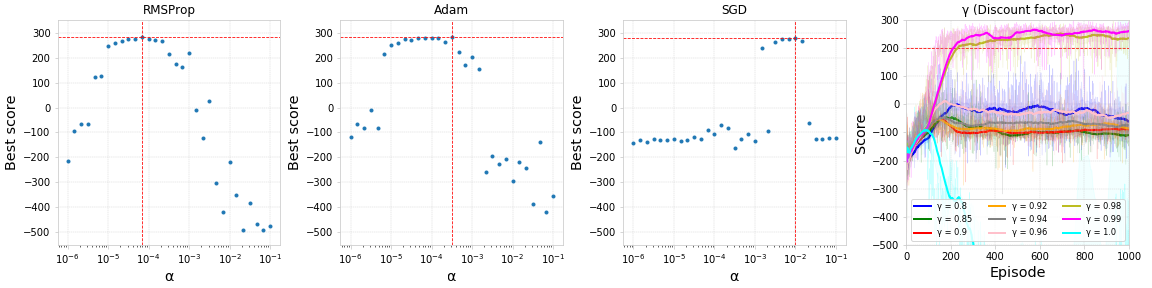
\includegraphics[width=\textwidth]{./images/fig3.png}
        \centering
        \caption{First 3 charts show best score achieved by integrated agent over 1000 episodes using different optimization algorithms and learning rates, while chart in the right shows score evolution over 1000 episodes for different discount factors.}
        \label{fig:fig3}
    \end{figure}

    Figure \ref{fig:fig3} presents experiment 2 and 3.
    All optimization algorithms produced comparable best performances: RMSProp best result was 282 score for $\alpha = 6.8 \times 10^{-5}$, Adaptive Moment Estimation (Adam) best result was 281 score for $\alpha = 3.2 \times 10^{-4}$, and Stochastic Gradient Descent (SGD) best result was 277 for $\alpha = 10^{-2}$.

    An interesting observation can be made regarding how many tested learning rates provided scores above 200.
    13 out of 30 tested learning rates achieved results above 200 score for Adam algorithm;
    11 in the case of RMSProp;
    and only 6 in the case of SGD.
    This broader range of learning rates with superior performance for Adam and RMSProp in comparison to SGD suggests that those two algorithms should be preferred over SGD, which confirms our expectation.

    In figure \ref{fig:fig3} we can also see the impact of discount factor in agent's convergence.
    From the different discount factors tested, only $\gamma = 0.98$ and $\gamma = 0.99$ enabled the integrated agent to solve the Lunar Lander environment, converging to scores above 200.

    \begin{figure}[h]
        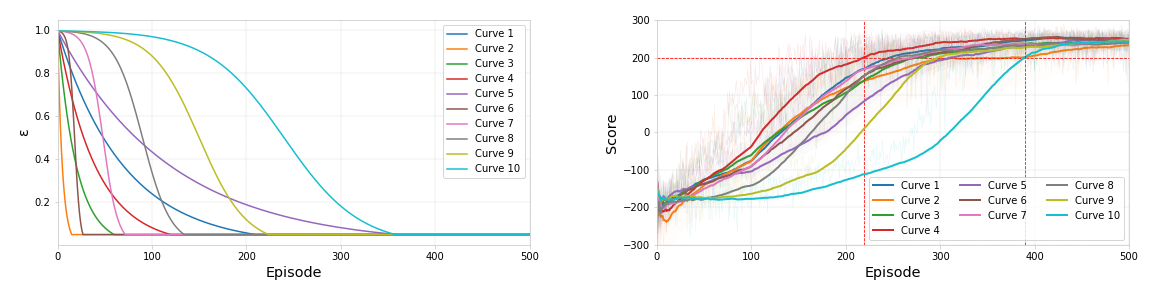
\includegraphics[width=\textwidth]{./images/fig4.png}
        \centering
        \caption{Impact of different exploration strategies in agent's learning.
        In the left, we show 10 different $\epsilon$-decay curves used, while in the right we show the effect of each of these curves in the integrated agent's performance.}
        \label{fig:fig4}
    \end{figure}

    Results from our final experiment are present in figure \ref{fig:fig4}.
    All exploration strategies enabled the integrated agent to converge and solve Lunar Lander environment regardless of their $\epsilon$-decay curve format, as expected.
    However, some exploration strategies converged much faster.
    Curve 4, described by $\epsilon(t) = e^{-t / 40}$, showed the best result, making the agent achieve 200 score over 100-episodes rolling average in 219 episodes.
    Curve 10, described by $\epsilon(t) = 1 / (1 + e^{t/40 - 6})$, showed the worst result, converging in 390 episodes.
    Curiously, curves 2, 3 and 6, which decay $\epsilon$ more aggressively than curve 4, performed worse than the best curve.
    This observation is yet another occurrence of something noted in several experiments: the best performing hyper-parameter is never at extremes.

    \section{Conclusion}
    \label{sec:conclusion}

    In this work, we implemented Deep Q-Networks and some of their main extensions (Double Q-learning, Dueling Networks, and Prioritized Experience Replay), studying their performance in Lunar Lander environment from OpenAI gym.
    We were able to confirm several points made in the articles that introduced DQN and their extensions.
    Our experiments achieved results that would put our implemented agents in top 2nd position in the \href{https://github.com/openai/gym/wiki/Leaderboard#lunarlander-v2}{leaderboard}.

\printbibliography

\end{document}
